%%%%%%%%%%%%%%%%%%%%%%%%%%%%%%%%%%%%%%%%%
% baposter Portrait Poster
% LaTeX Template
% Version 1.0 (15/5/13)
%
% Created by:
% Brian Amberg (baposter@brian-amberg.de)
%
% This template has been downloaded from:
% http://www.LaTeXTemplates.com
%
% License:
% CC BY-NC-SA 3.0 (http://creativecommons.org/licenses/by-nc-sa/3.0/)
%
%%%%%%%%%%%%%%%%%%%%%%%%%%%%%%%%%%%%%%%%%

%----------------------------------------------------------------------------------------
%	PACKAGES AND OTHER DOCUMENT CONFIGURATIONS
%----------------------------------------------------------------------------------------

\documentclass[a0paper,portrait]{baposter}

\usepackage[font=small,labelfont=bf]{caption} % Required for specifying captions to tables and figures
\usepackage{booktabs} % Horizontal rules in tables
\usepackage{relsize} % Used for making text smaller in some places
\usepackage{tikz}
\usepackage{pgf-pie}
\usepackage{smartdiagram}

\usepackage{helvet}
\renewcommand{\familydefault}{\sfdefault}

\graphicspath{{figures/}} % Directory in which figures are stored

\definecolor{bordercol}{RGB}{40,40,40} % Border color of content boxes
\definecolor{headercol1}{RGB}{186,215,230} % Background color for the header in the content boxes (left side)
\definecolor{headercol2}{RGB}{80,80,80} % Background color for the header in the content boxes (right side)
\definecolor{headerfontcol}{RGB}{0,0,0} % Text color for the header text in the content boxes
\definecolor{boxcolor}{RGB}{186,215,230} % Background color for the content in the content boxes

\begin{document}

\background{ % Set the background to an image (background.pdf)
\begin{tikzpicture}[remember picture,overlay]
\draw (current page.north west)+(-2em,2em) node[anchor=north west]
{\includegraphics[height=1.1\textheight]{background}};
\end{tikzpicture}
}

\begin{poster}{
grid=false,
borderColor=bordercol, % Border color of content boxes
headerColorOne=headercol1, % Background color for the header in the content boxes (left side)
headerColorTwo=headercol2, % Background color for the header in the content boxes (right side)
headerFontColor=headerfontcol, % Text color for the header text in the content boxes
boxColorOne=boxcolor, % Background color for the content in the content boxes
headershape=roundedright, % Specify the rounded corner in the content box headers
headerfont=\Large\sf\bf, % Font modifiers for the text in the content box headers
textborder=rectangle,
background=user,
headerborder=open, % Change to closed for a line under the content box headers
boxshade=plain,
headerheight=0.16\textheight
}
{}
%
%----------------------------------------------------------------------------------------
%	TITLE AND AUTHOR NAME
%----------------------------------------------------------------------------------------
%
{\sf\bf Diabetic Retinopathy Detection through Image Analysis Using Deep Convolutional Neural Networks} % Poster title
{\vspace{1em} Jordi de la Torre, Aida Valls and Domenec Puig\\ % Author names
Departament d'Enginyeria Inform\`atica i Matem\`atiques\\
Universitat Rovira i Virgili\\
{\smaller jordi.delatorre@gmail.com, aida.valls@urv.cat, domenec.puig@urv.cat}} % Author email addresses
{
\includegraphics[scale=0.50]{logo}} % University/lab logo

%----------------------------------------------------------------------------------------
%	INTRODUCTION
%----------------------------------------------------------------------------------------

\headerbox{Introduction}{name=introduction,column=0,row=0}{

Diabetic Retinopathy (DR) is a leading disabling chronic disease  and  one of the main causes of blindness and visual impairment in developed countries for diabetic patients. Ninety percent of the cases can be prevented through early detection and treatment. Eye screening through retinal images is used by physicians to detect the lesions related with this disease. 

}
%----------------------------------------------------------------------------------------
%	MATERIALS AND METHODS
%----------------------------------------------------------------------------------------

\headerbox{Data}{name=methods,column=0,below=introduction}{
\begin{center}
	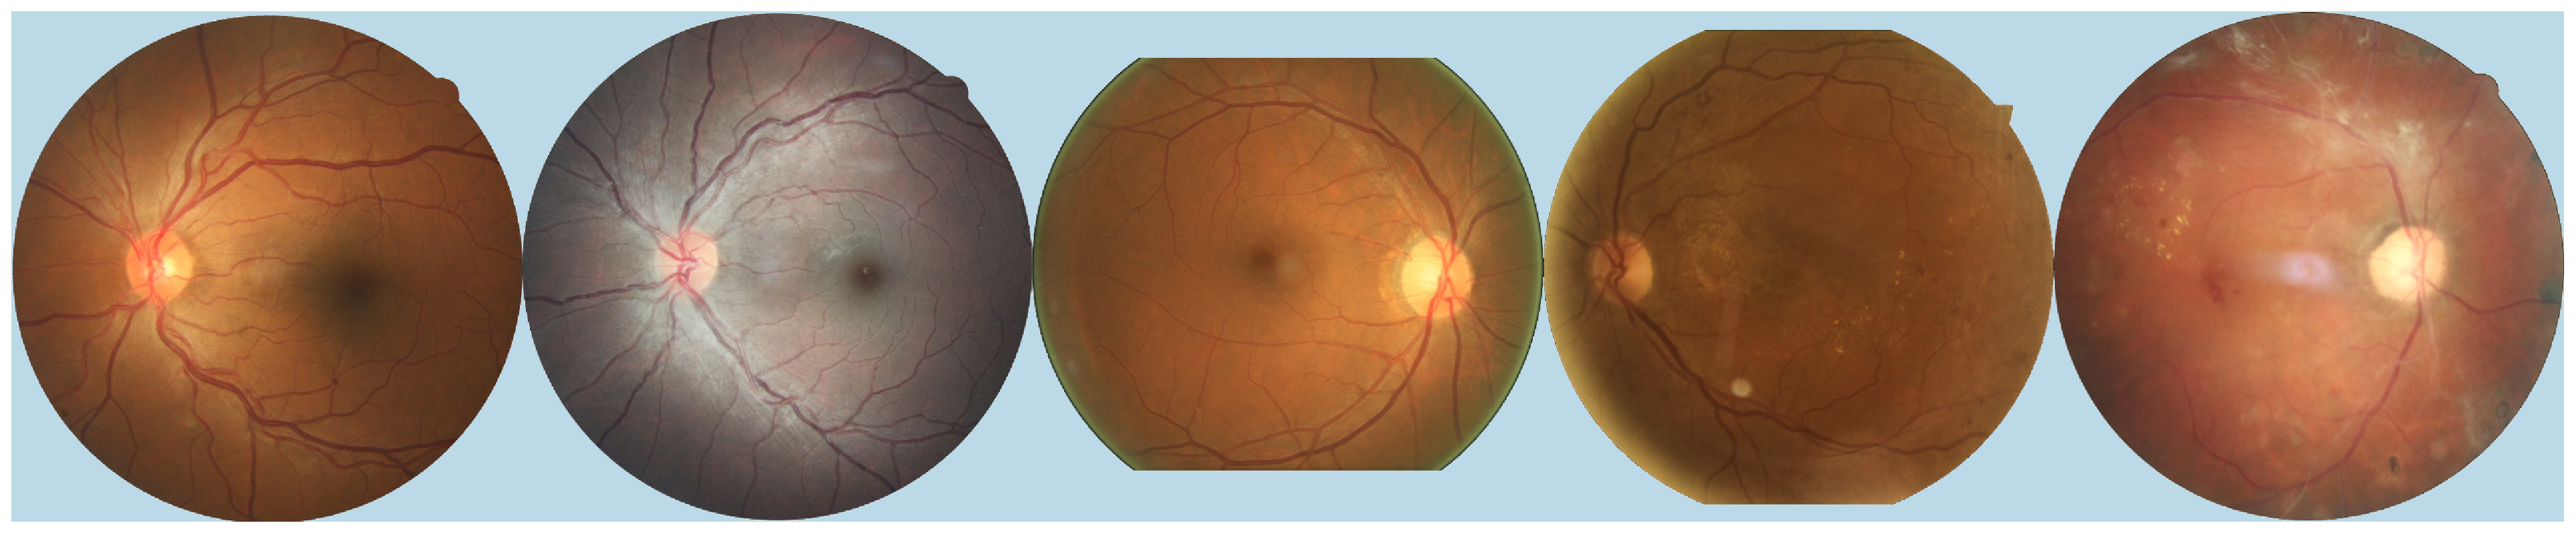
\includegraphics[width=0.99\textwidth]{5-classes.eps}
	\captionof{figure}{Five classes to predict. Class 0 (no apparent retinopathy), Class 1 (Mild), Class 2 (Moderate),Class 3 (Severe), Class 4 (Proliferative).}
\end{center}

\begin{center}
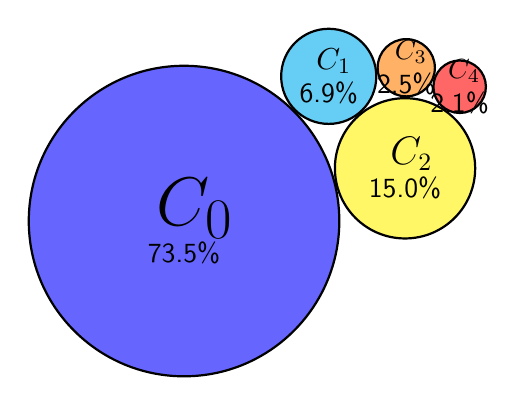
\begin{tikzpicture}[scale=0.23]
\pie[cloud, text=inside,scale font, radius=10]
{
	73.5/ $C_0$,
	6.9/ $C_1$,
	15.0/ $C_2$,
	2.5/ $C_3$,
	2.1/ $C_4$
}
\end{tikzpicture}
\captionof{figure}{Class distribution of the dataset}
\end{center}


\begin{center}
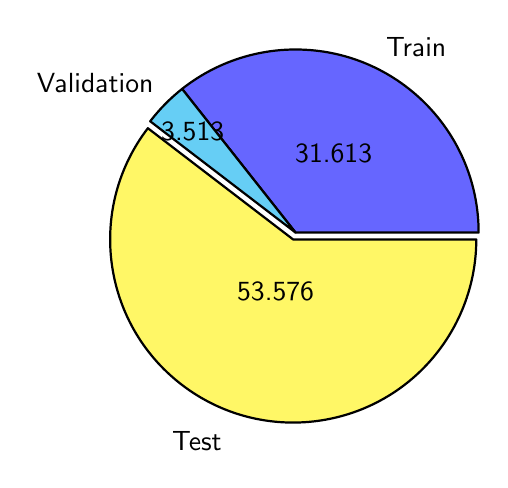
\begin{tikzpicture}[scale = 0.93]
\pie[sum=auto , after  number=, radius = 2.5, explode={0, 0, 0.1}]{31.613/Train, 3.513/Validation,  53.576/Test}
\end{tikzpicture}
\captionof{figure}{Training, Validation and Testing sets}
\end{center}

}

%----------------------------------------------------------------------------------------
%	CONCLUSION
%----------------------------------------------------------------------------------------

\headerbox{Conclusions}{name=conclusion,column=0,below=methods}{

In this paper we show that deep learning techniques are a promising technique for solving medical imaging problems like the diabetic retinopathy detection. Having enough data this method is able to perform near human level expertise achieving $\kappa$ values of 0.752 not far from the $\kappa$ achieved by human experts, around 0.800. 
}

%----------------------------------------------------------------------------------------
%	ACKNOWLEDGEMENTS
%----------------------------------------------------------------------------------------

\headerbox{Forthcomming research}{name=forthcomming,column=0,below=conclusion, above=bottom}{
Future work will be centered on testing higher resolution input images, newer schemes, alternative cost functions and more elaborated methods for combining the information coming from both eyes.
} 

\headerbox{Train}{name=train,column=1,row=0}{ % To reduce this block to 1 column width, remove 'span=2'
	\begin{center}
		\includegraphics[scale=0.92]{training-crop.pdf}
		\captionof{figure}{Training procedure: online data augmentation plus model optimization}
	\end{center}
}

\headerbox{Best Model}{name=test,column=2,row=0}{ % To reduce this block to 1 column width, remove 'span=2'
	\begin{center}
		\includegraphics[scale=0.84]{nnarch-crop.pdf}
		\captionof{figure}{Architecture of the model with best performance}
	\end{center}
}

\headerbox{Test}{name=test,span=2,column=1,below=train,above=bottom}{ % To reduce this block to 1 column width, remove 'span=2'
	\begin{center}
		\includegraphics[scale = 0.58]{testing-crop.pdf}
		\captionof{figure}{Geometric mean of five evaluations of the same rotated image}
		\includegraphics[scale = 0.64]{combination-crop.pdf}
		\captionof{figure}{Method for combining the information coming from both eyes to improve the classification}
	\end{center}
}



%----------------------------------------------------------------------------------------

\end{poster}

\end{document}